\setbeamercolor{background canvas}{bg=fitblue}
\begin{frame}
  \frametitle{Shadow Mapping}
  \begin{center}
    \Huge {\color{white}Shadow Mapping}
  \end{center}
\end{frame}
\setbeamercolor{background canvas}{bg=white}

\begin{frame}
  \frametitle{Shadow-Mapping - přehled}
  \begin{itemize}
    \item Dva průchody
    \item Dva druhy vzorků \\ (view-samples, shadow-samples)
    \item Každý view-sample má přiřazený \\ shadow-sample
  \end{itemize}
  \begin{picture}(320,250)
    \put(135,120){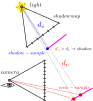
\includegraphics[height=7.5cm,keepaspectratio]{pics/shadows/shadowMapping/shadowmapping}}
    \put(-20,100 ){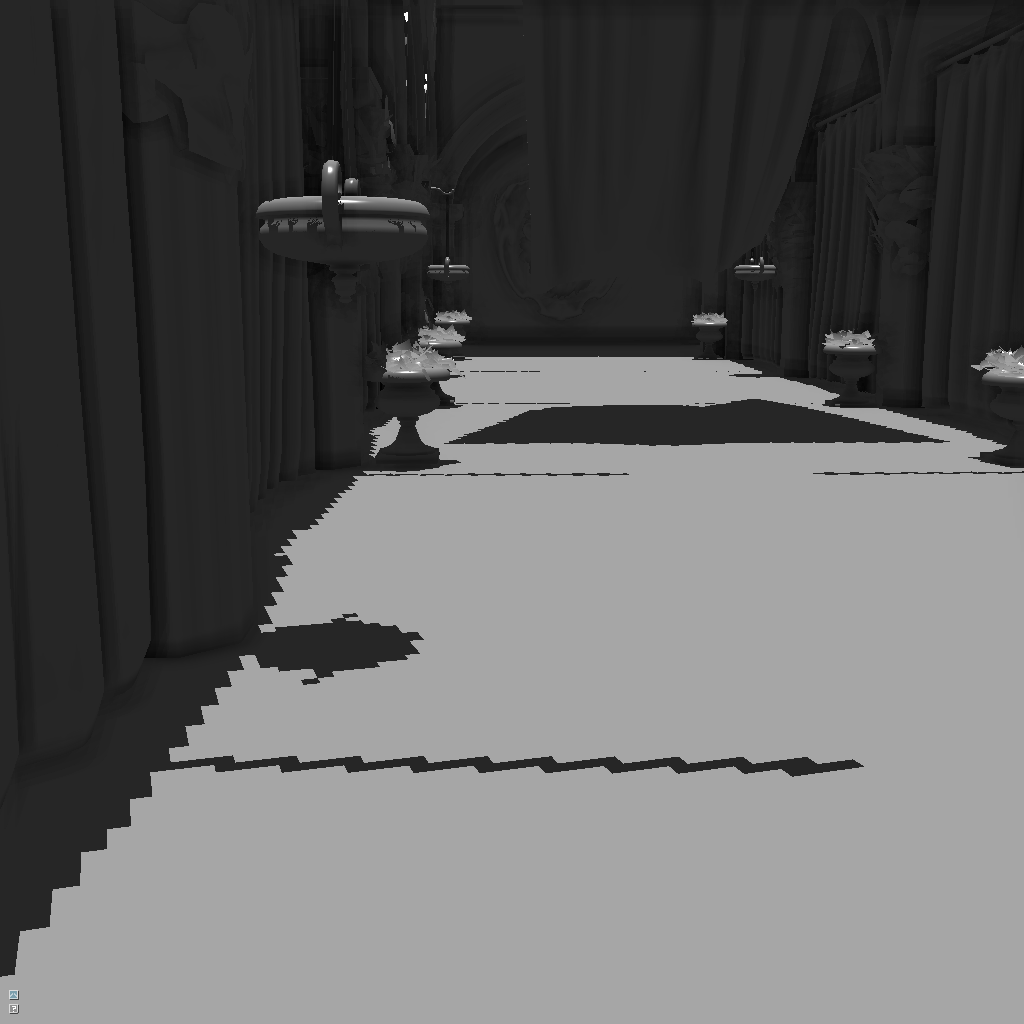
\includegraphics[height=5cm,keepaspectratio]{pics/shadows/shadowMapping/sponza2_sm}}
  \end{picture}
\end{frame}



\begin{frame}
    \frametitle{Stínové mapy}

%    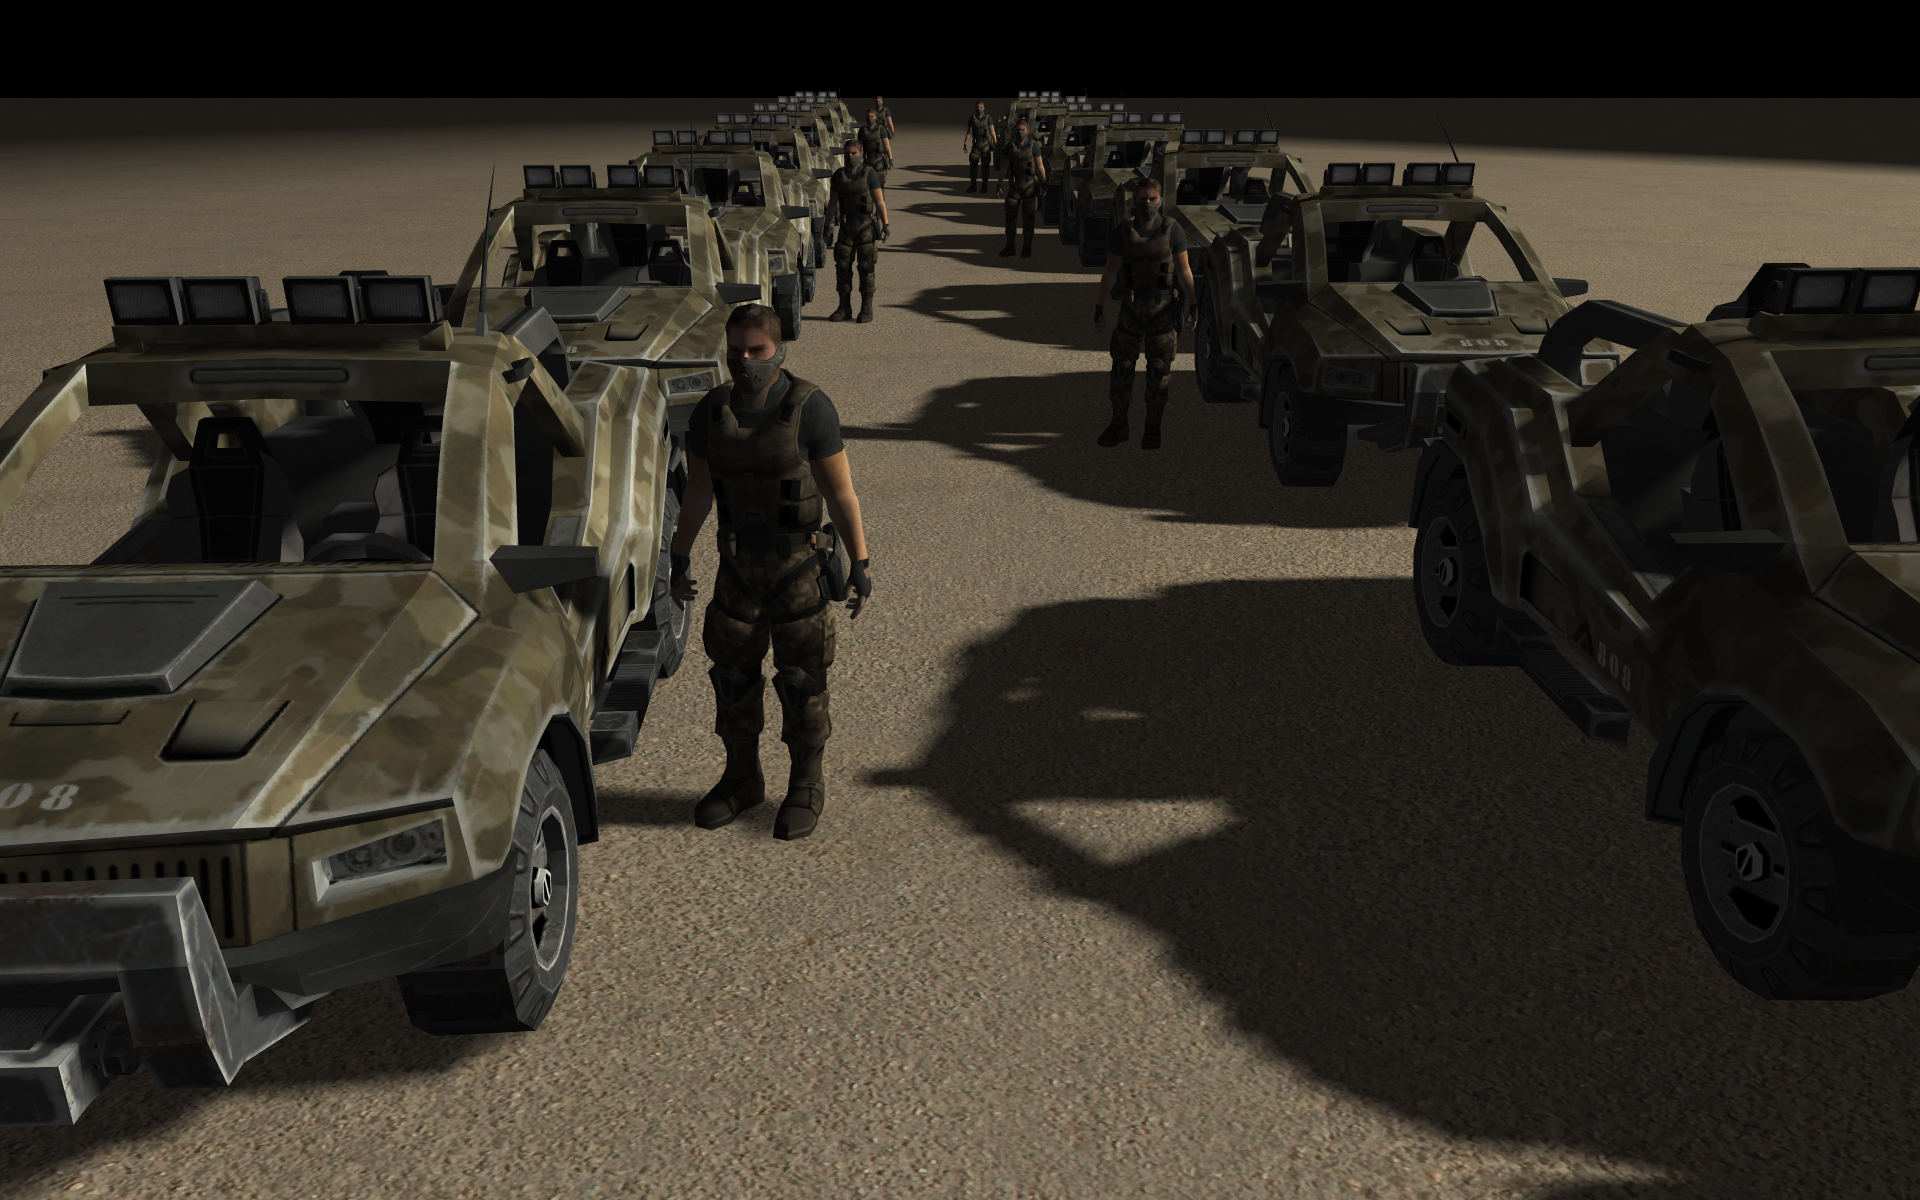
\includegraphics[width=\textwidth]{pics/shadows/shadowMapping/vsm.eps}
    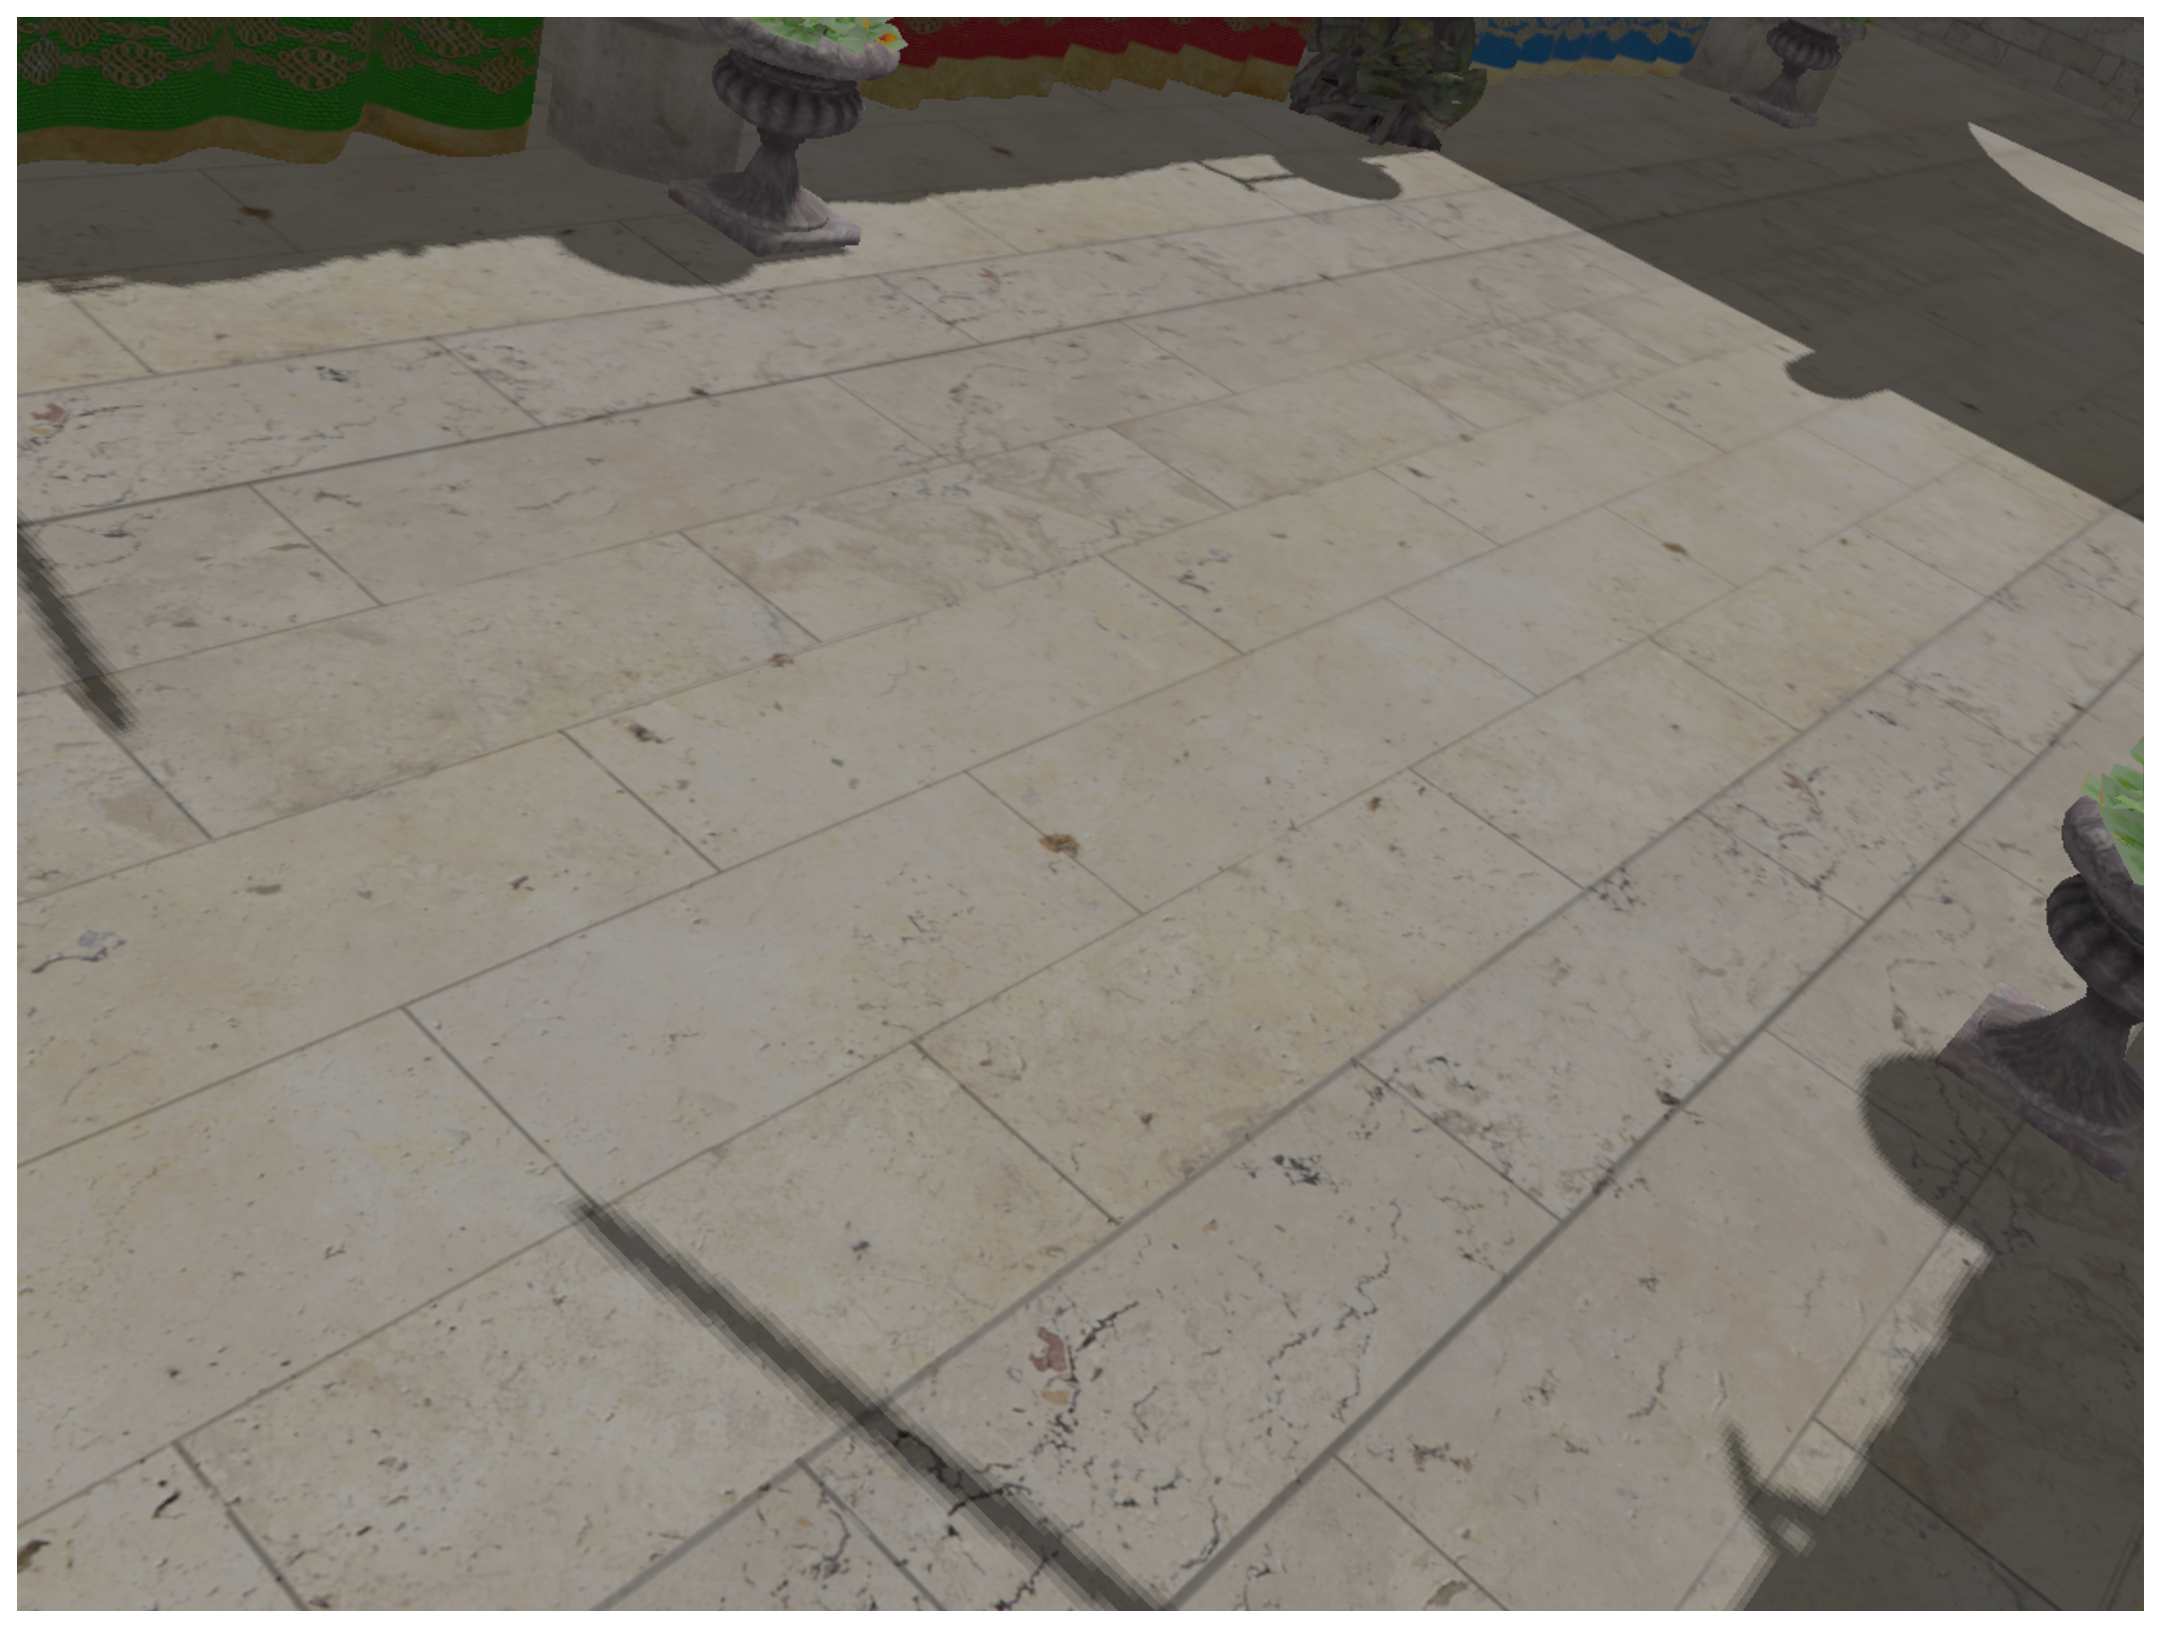
\includegraphics[width=\textwidth]{pics/shadows/shadowMapping/pcf_nearest.eps}
\end{frame}

\begin{frame}
    \frametitle{Princip}
    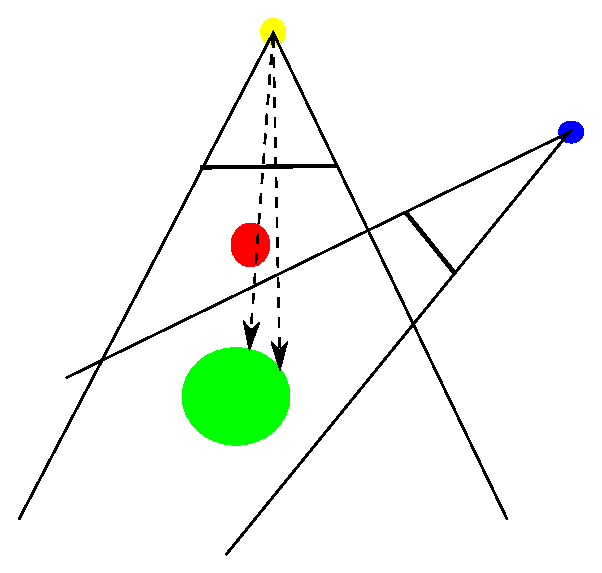
\includegraphics[height=.75\textheight]{pics/shadows/shadowMapping/smap.eps}
    \begin{itemize}
        \item Připravíme si z-buffer kamery ve světle.
        \item Porovnáváme hloubky vykreslovaných fragmentù.
    \end{itemize}
\end{frame}

\begin{frame}
    \frametitle{Hloubková mapa}
    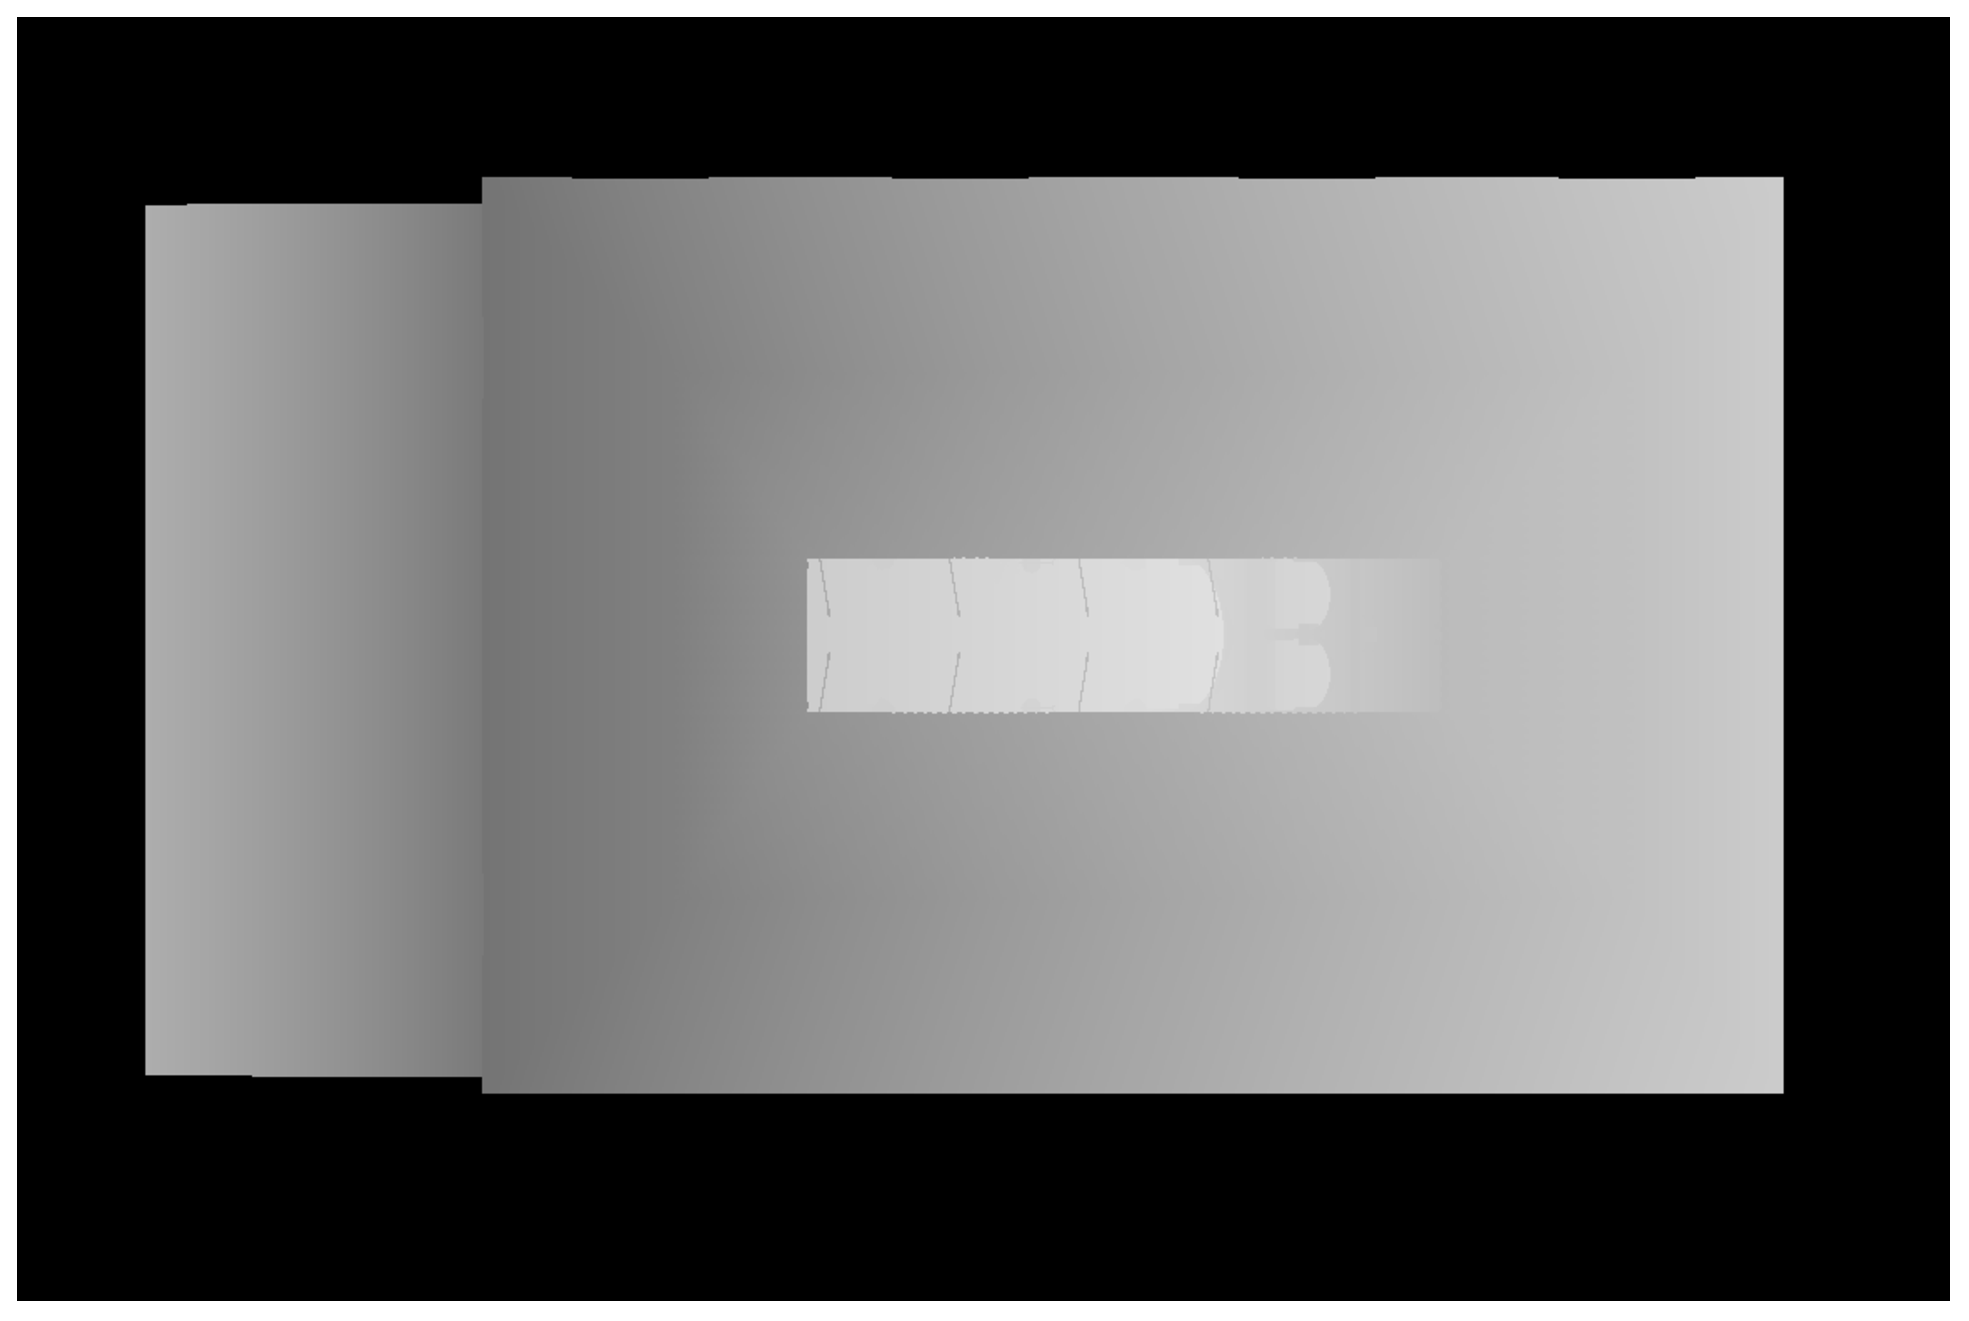
\includegraphics[width=\textwidth]{pics/shadows/shadowMapping/depth.eps}
\end{frame}


\begin{frame}
    \frametitle{Matika stínových těles}

    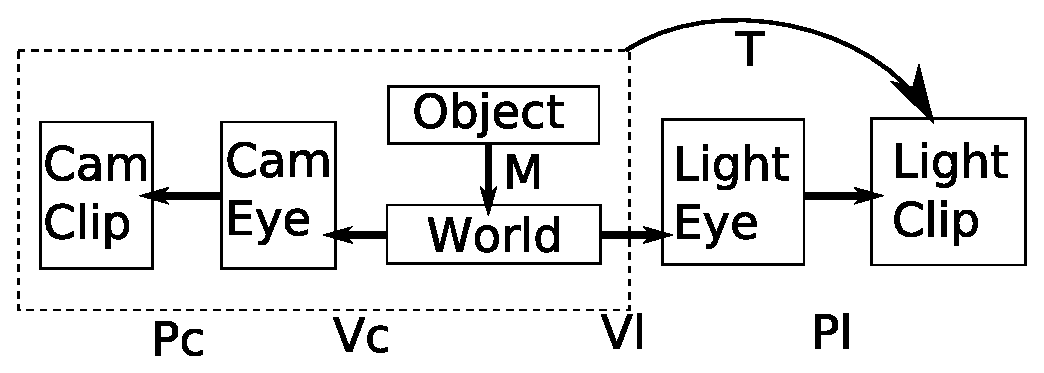
\includegraphics[width=4in]{pics/shadows/shadowMapping/smspc.eps}
    
    \vfill

    $\displaystyle T = \left( \begin{array}{cccc}
        0.5 & 0   & 0   & 0.5 \\
        0   & 0.5 & 0   & 0.5 \\
        0   & 0   & 0.5 & 0.5 \\
        0   & 0   & 0   & 1 \end{array} \right) \cdot P_l \cdot V_l \cdot M$
\end{frame}

\begin{frame}[fragile]
    \frametitle{GLSL}

{\small
  \begin{minted}[frame=lines]{glsl}
//Vertex shader
in vec4 position;
out vec4 shadowPos;
uniform mat4 shadowMat;
void main() {
    //...
    shadowPos = shadowMat*position;
    //...
}
//Fragment shader
in vec4 shadowPos;
uniform sampler2D shadow;
void main() {
    vec3 sp = shadowPos/shadowPos.w;
    if(texture(shadow, sp.xy).x < sp.z)
        gl_FragColor = shadowed_color;
    else
        gl_FragColor = unshadowed_color;
}
  \end{minted}
}
\end{frame}

\begin{frame}
    \frametitle{Shadow Acne}
    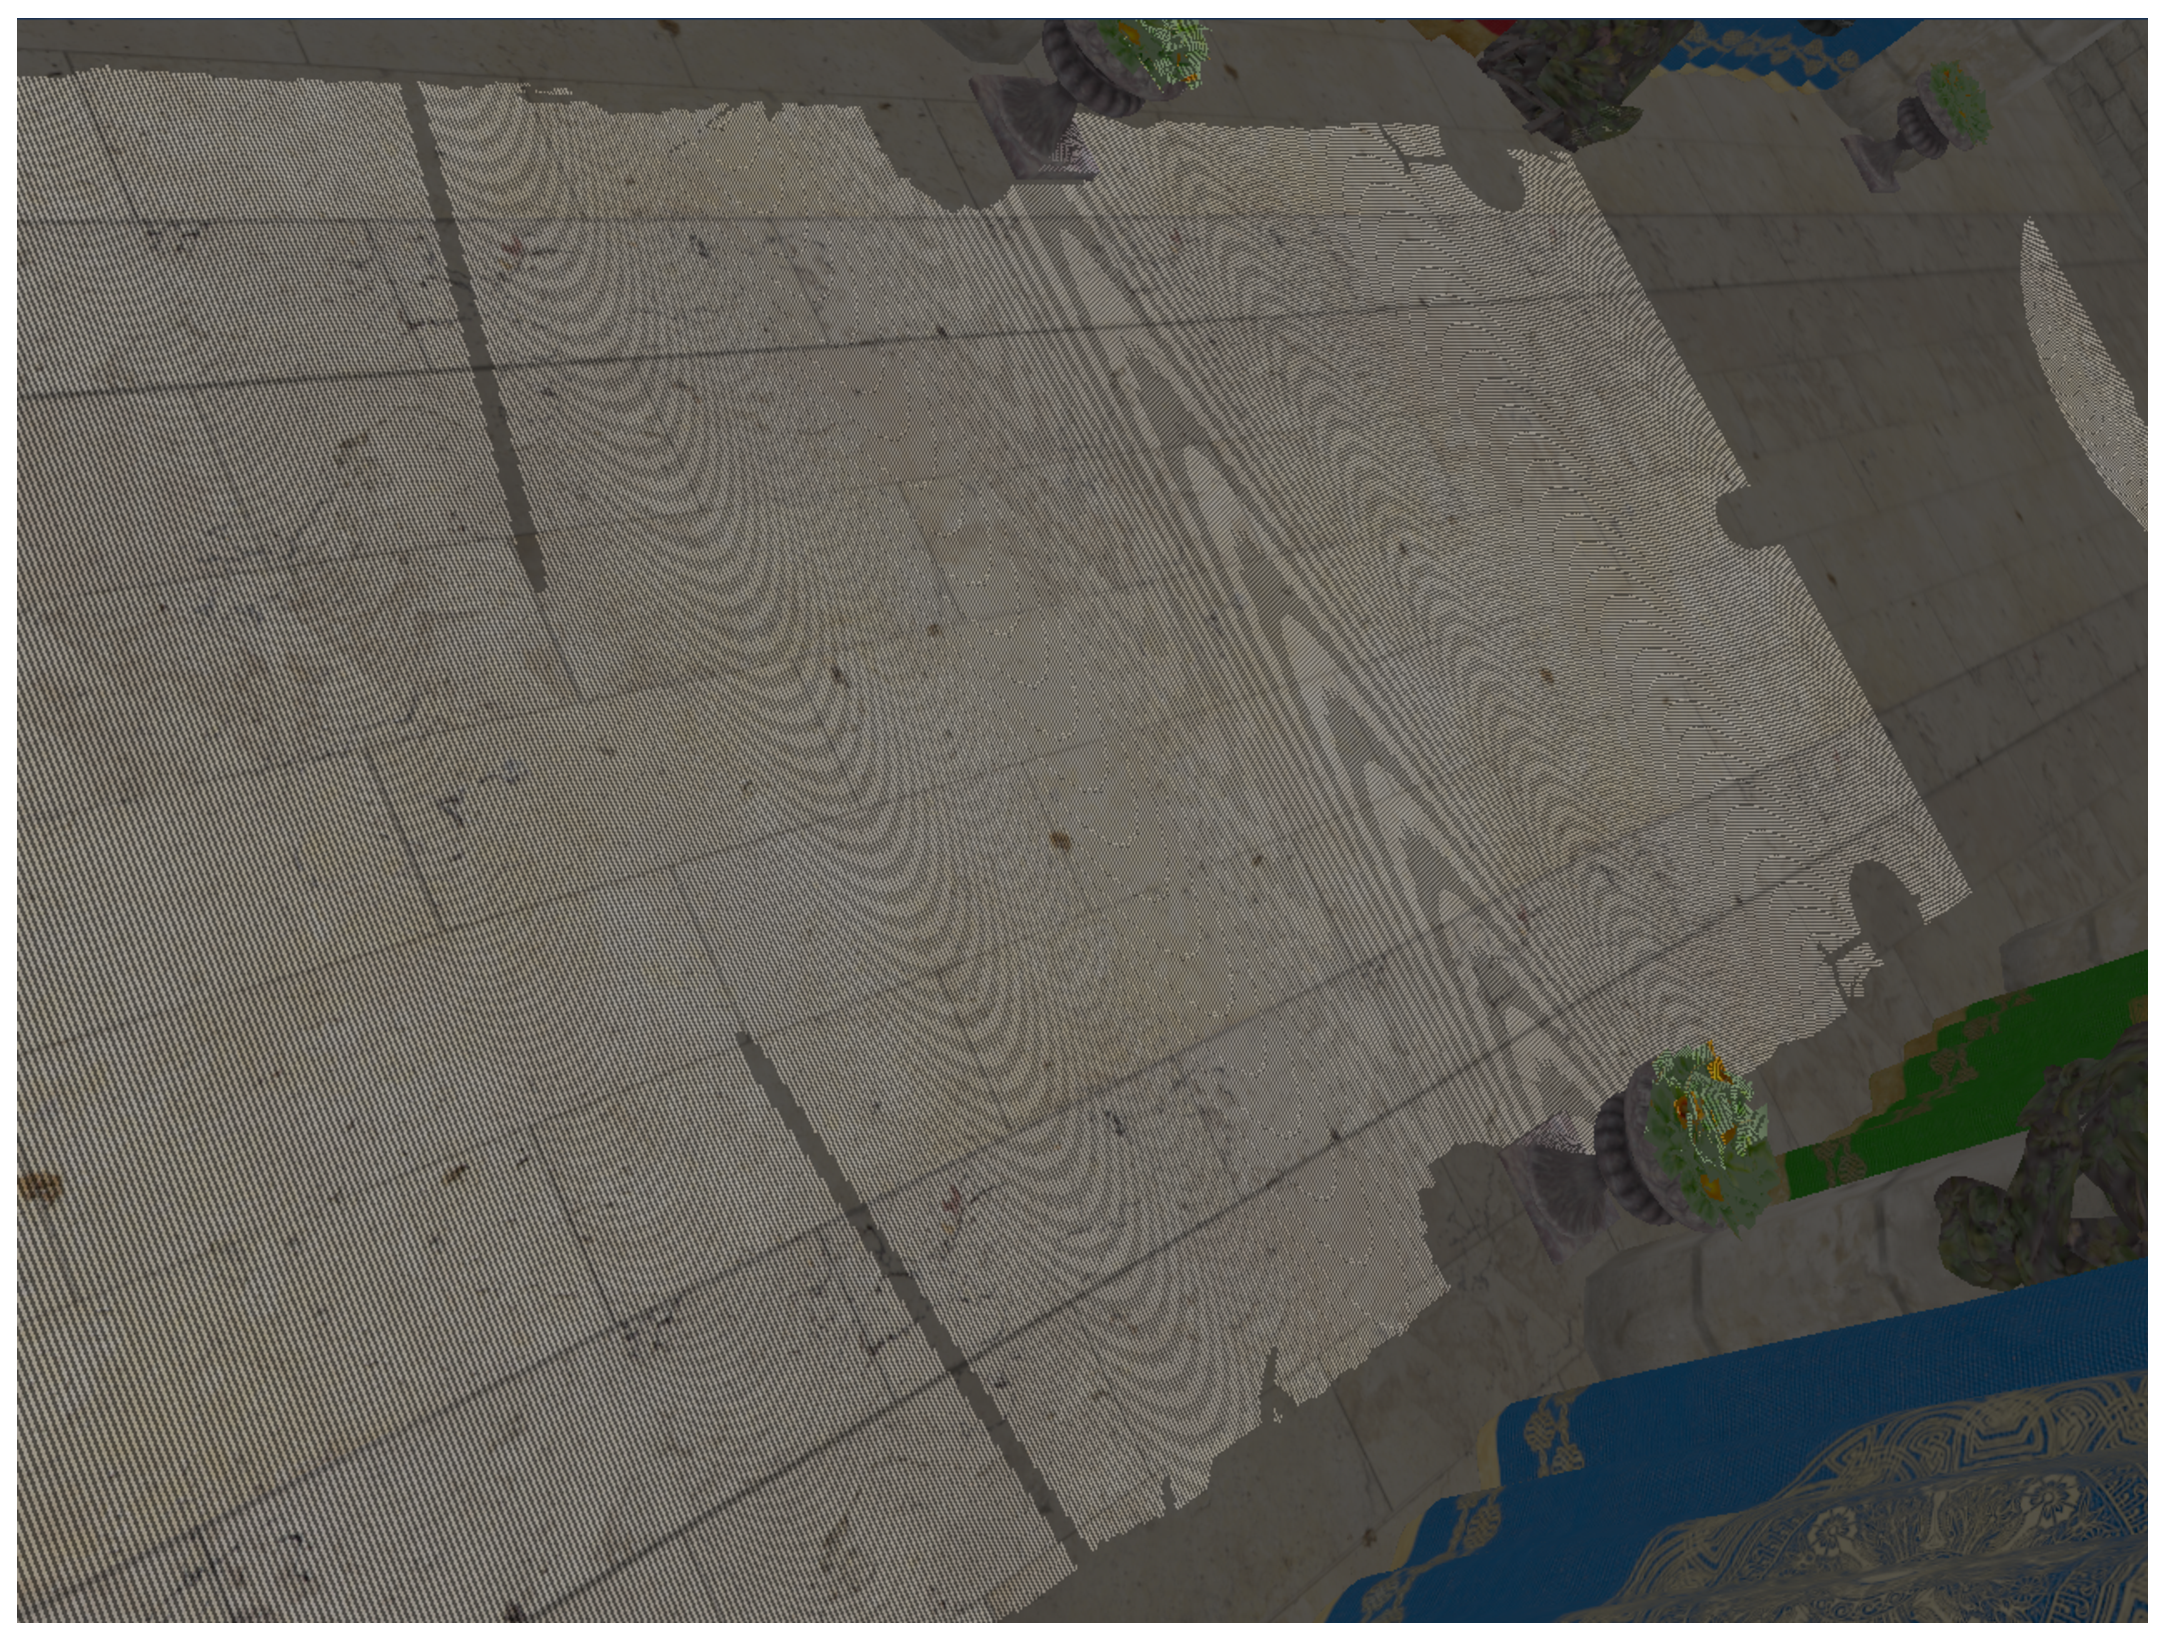
\includegraphics[width=\textwidth]{pics/shadows/shadowMapping/acne.eps}
\end{frame}

\begin{frame}[fragile]
    \frametitle{Bias}
    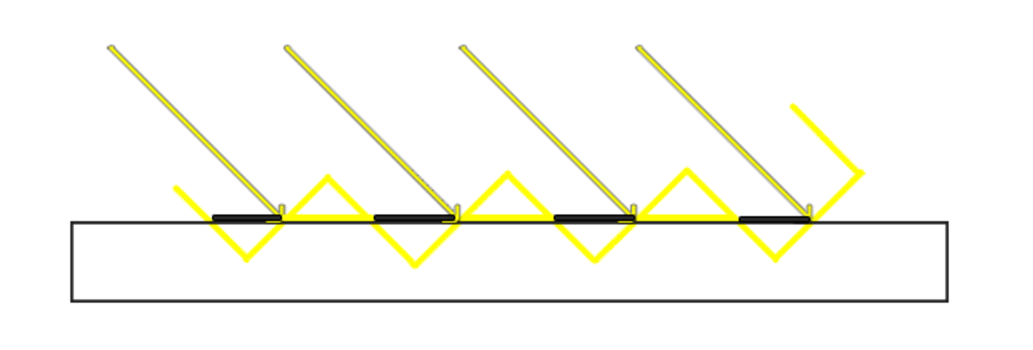
\includegraphics[width=.5\textwidth]{pics/shadows/shadowMapping/acne_before.eps}
    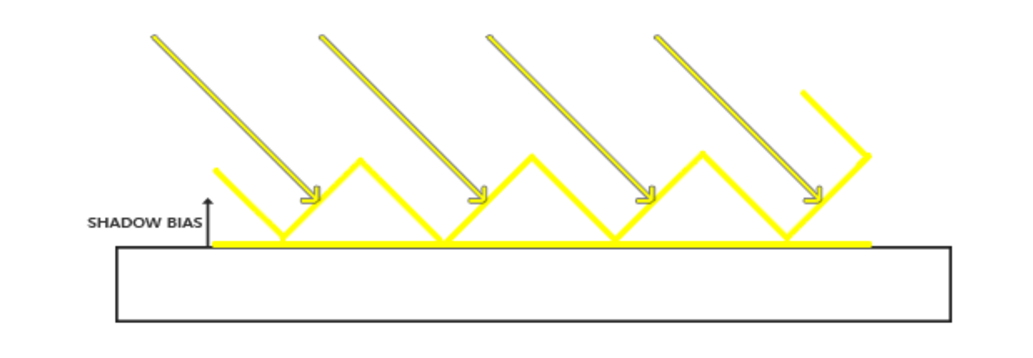
\includegraphics[width=.5\textwidth]{pics/shadows/shadowMapping/acne_after.eps}
    \vfill

{\small
  \begin{minted}[frame=lines]{glsl}
float depth = texture(shadowTexture, shadow_pos.xy).x;
float bias = max(0.05 * (1.0 - dot(N, L)), 0.005);
float shadow = shadow_pos.z - bias > depth ? 1.0 : 0.0; 
  \end{minted}
}
\end{frame}

\begin{frame}
    \frametitle{Alias}
    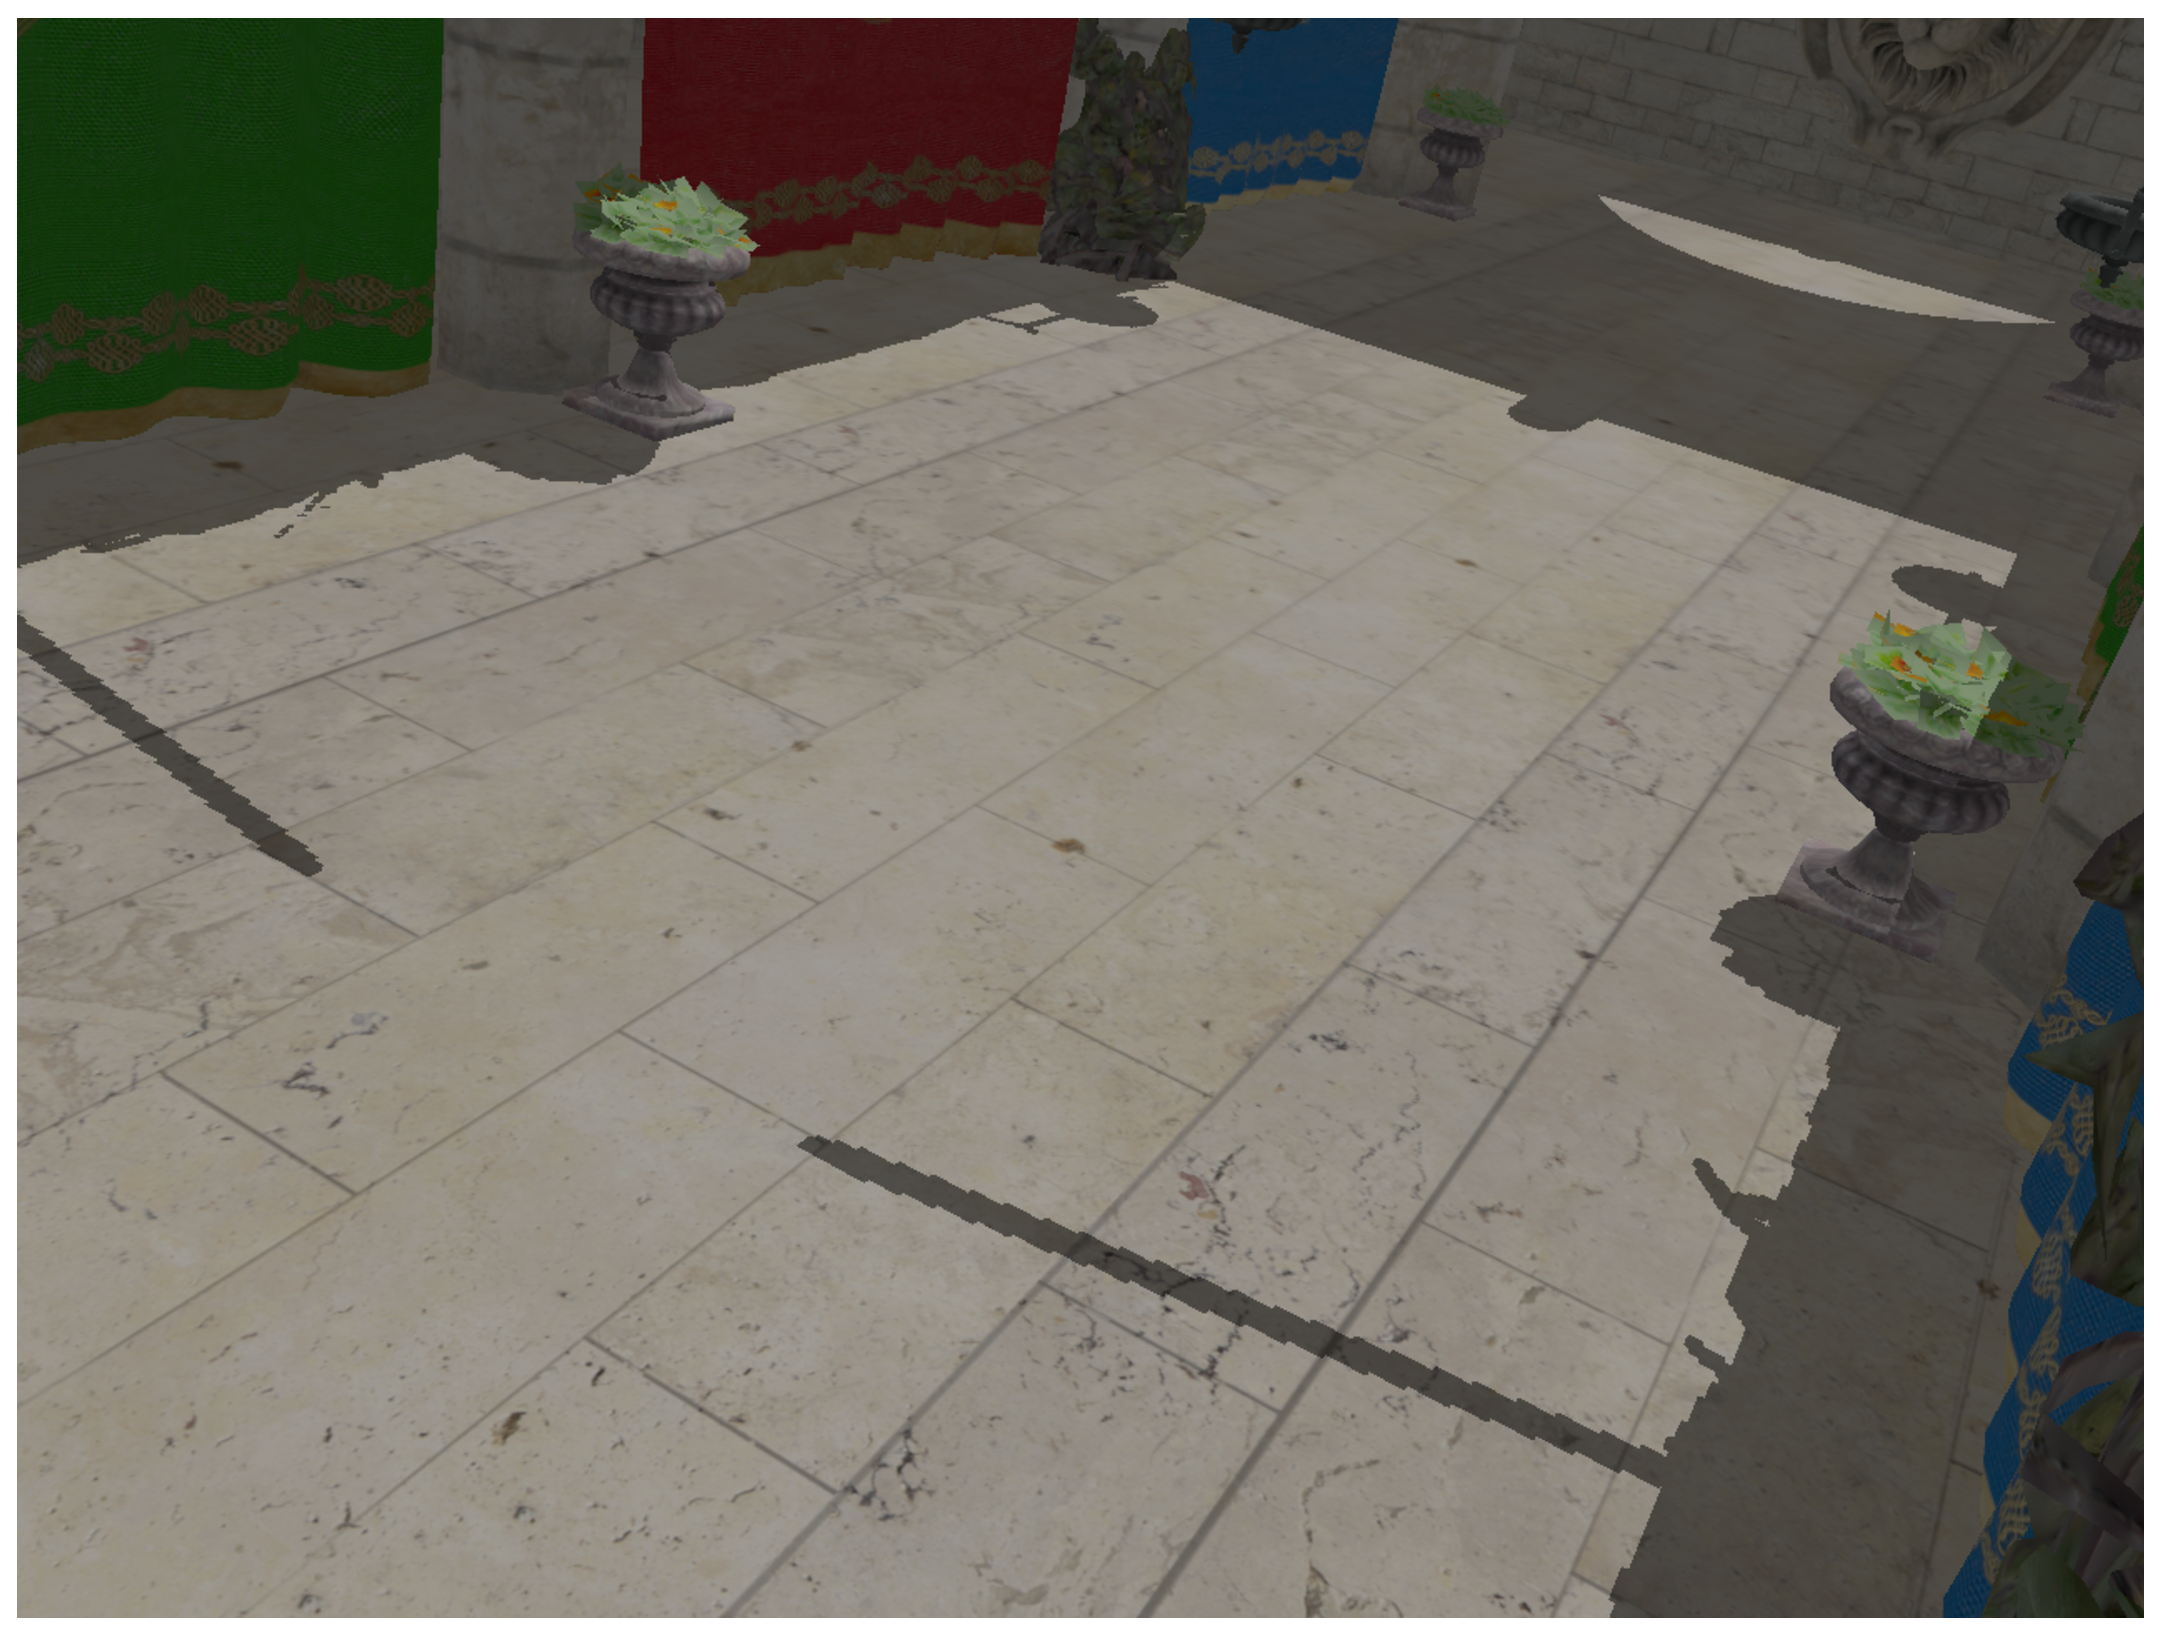
\includegraphics[width=\textwidth]{pics/shadows/shadowMapping/shadow_alias.eps}
\end{frame}

\begin{frame}
  \frametitle{Shadow-Mapping - Problems}
  \begin{itemize}
    \item Mnoho shadow-samples je nadužíváno.
    \item Mnoho shadow-samples není vůbec využito.
    \item $\to$ Zubaté hrany.
    \item Pro odstranění artefaktů je mnoho metod založeno na dělení prostoru nebo warpingu prostoru.
  \end{itemize}
  \begin{picture}(320,250)
    \put(-20,85){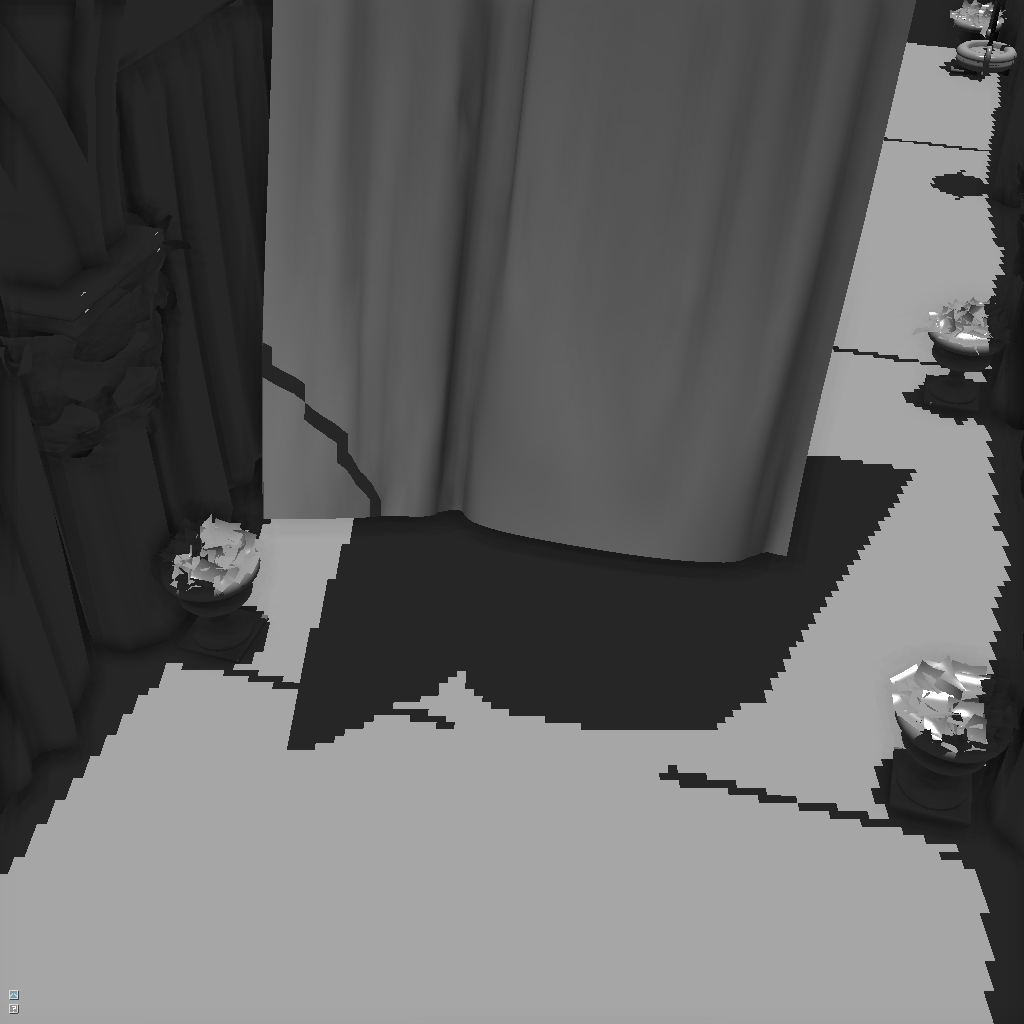
\includegraphics[height=5.5cm,keepaspectratio]{pics/shadows/shadowMapping/sponza_sm}}
    \put(160,85){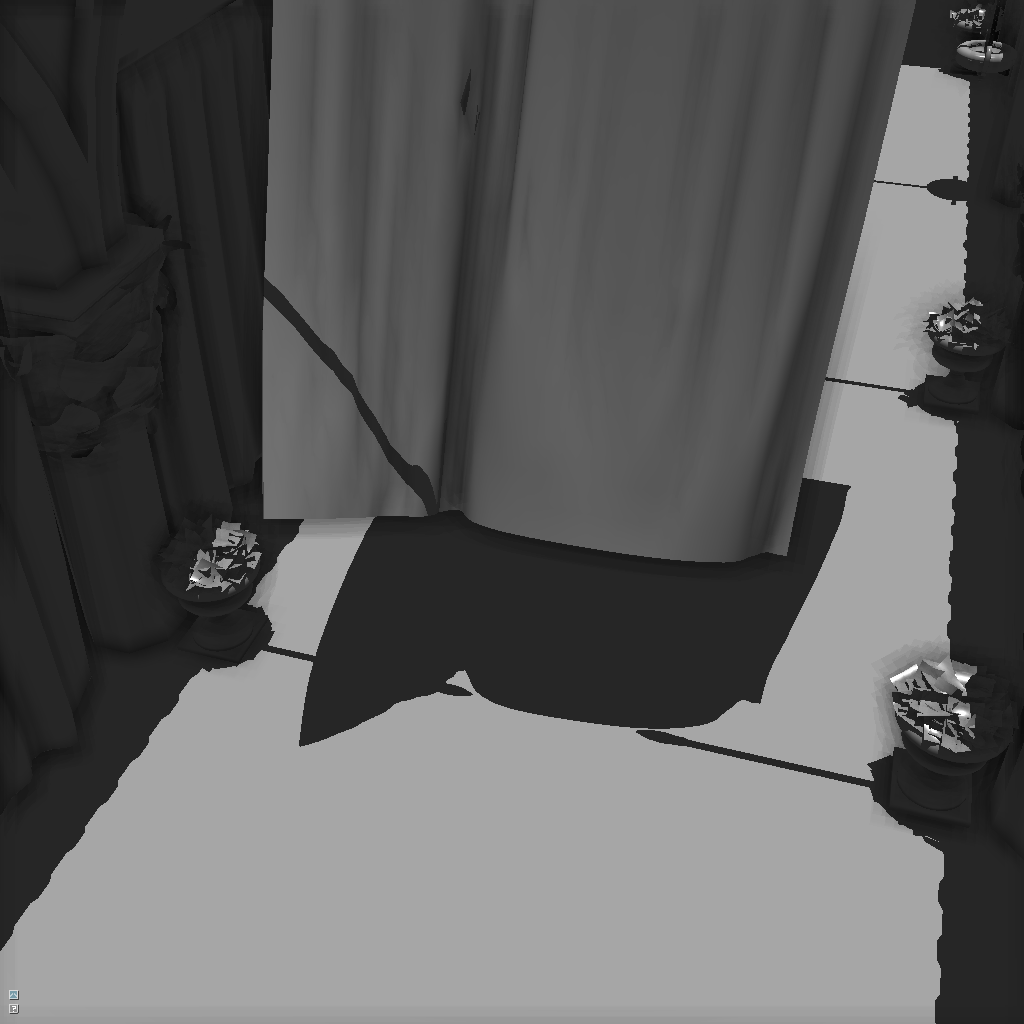
\includegraphics[height=5.5cm,keepaspectratio]{pics/shadows/shadowMapping/sponza_sv}}
  \end{picture}
\end{frame}

\begin{frame}
  \frametitle{Zubaté hrany}
  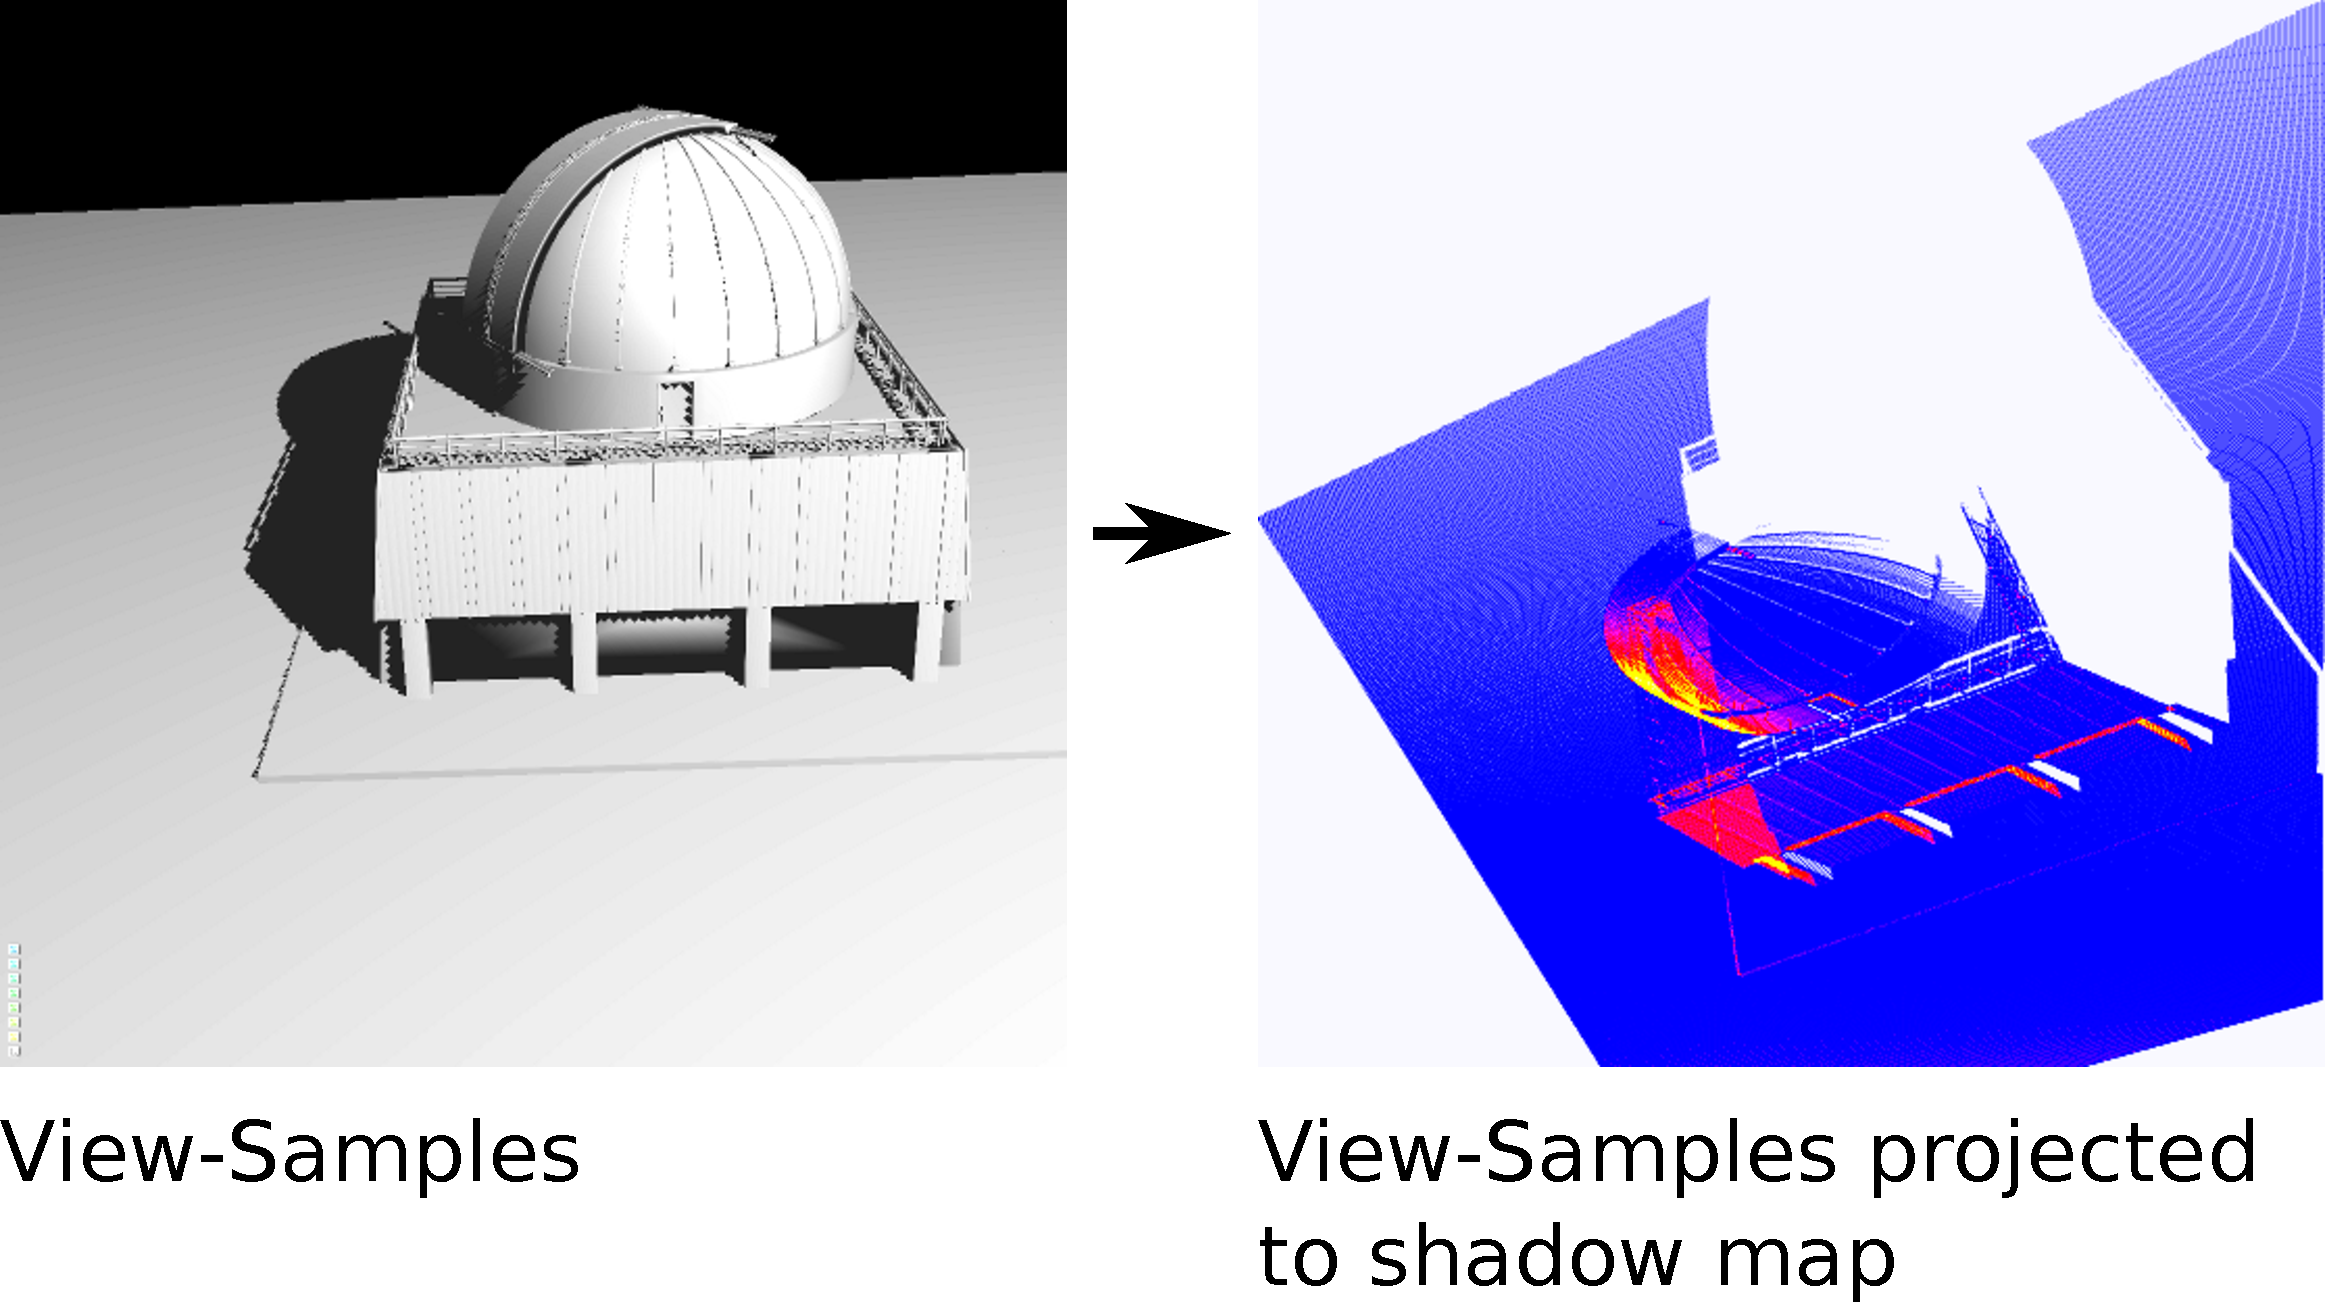
\includegraphics[width=\textwidth]{pics/shadows/shadowMapping/projectedShadowSamples}
\end{frame}

\begin{frame}
    \frametitle{Měkké stíny}
    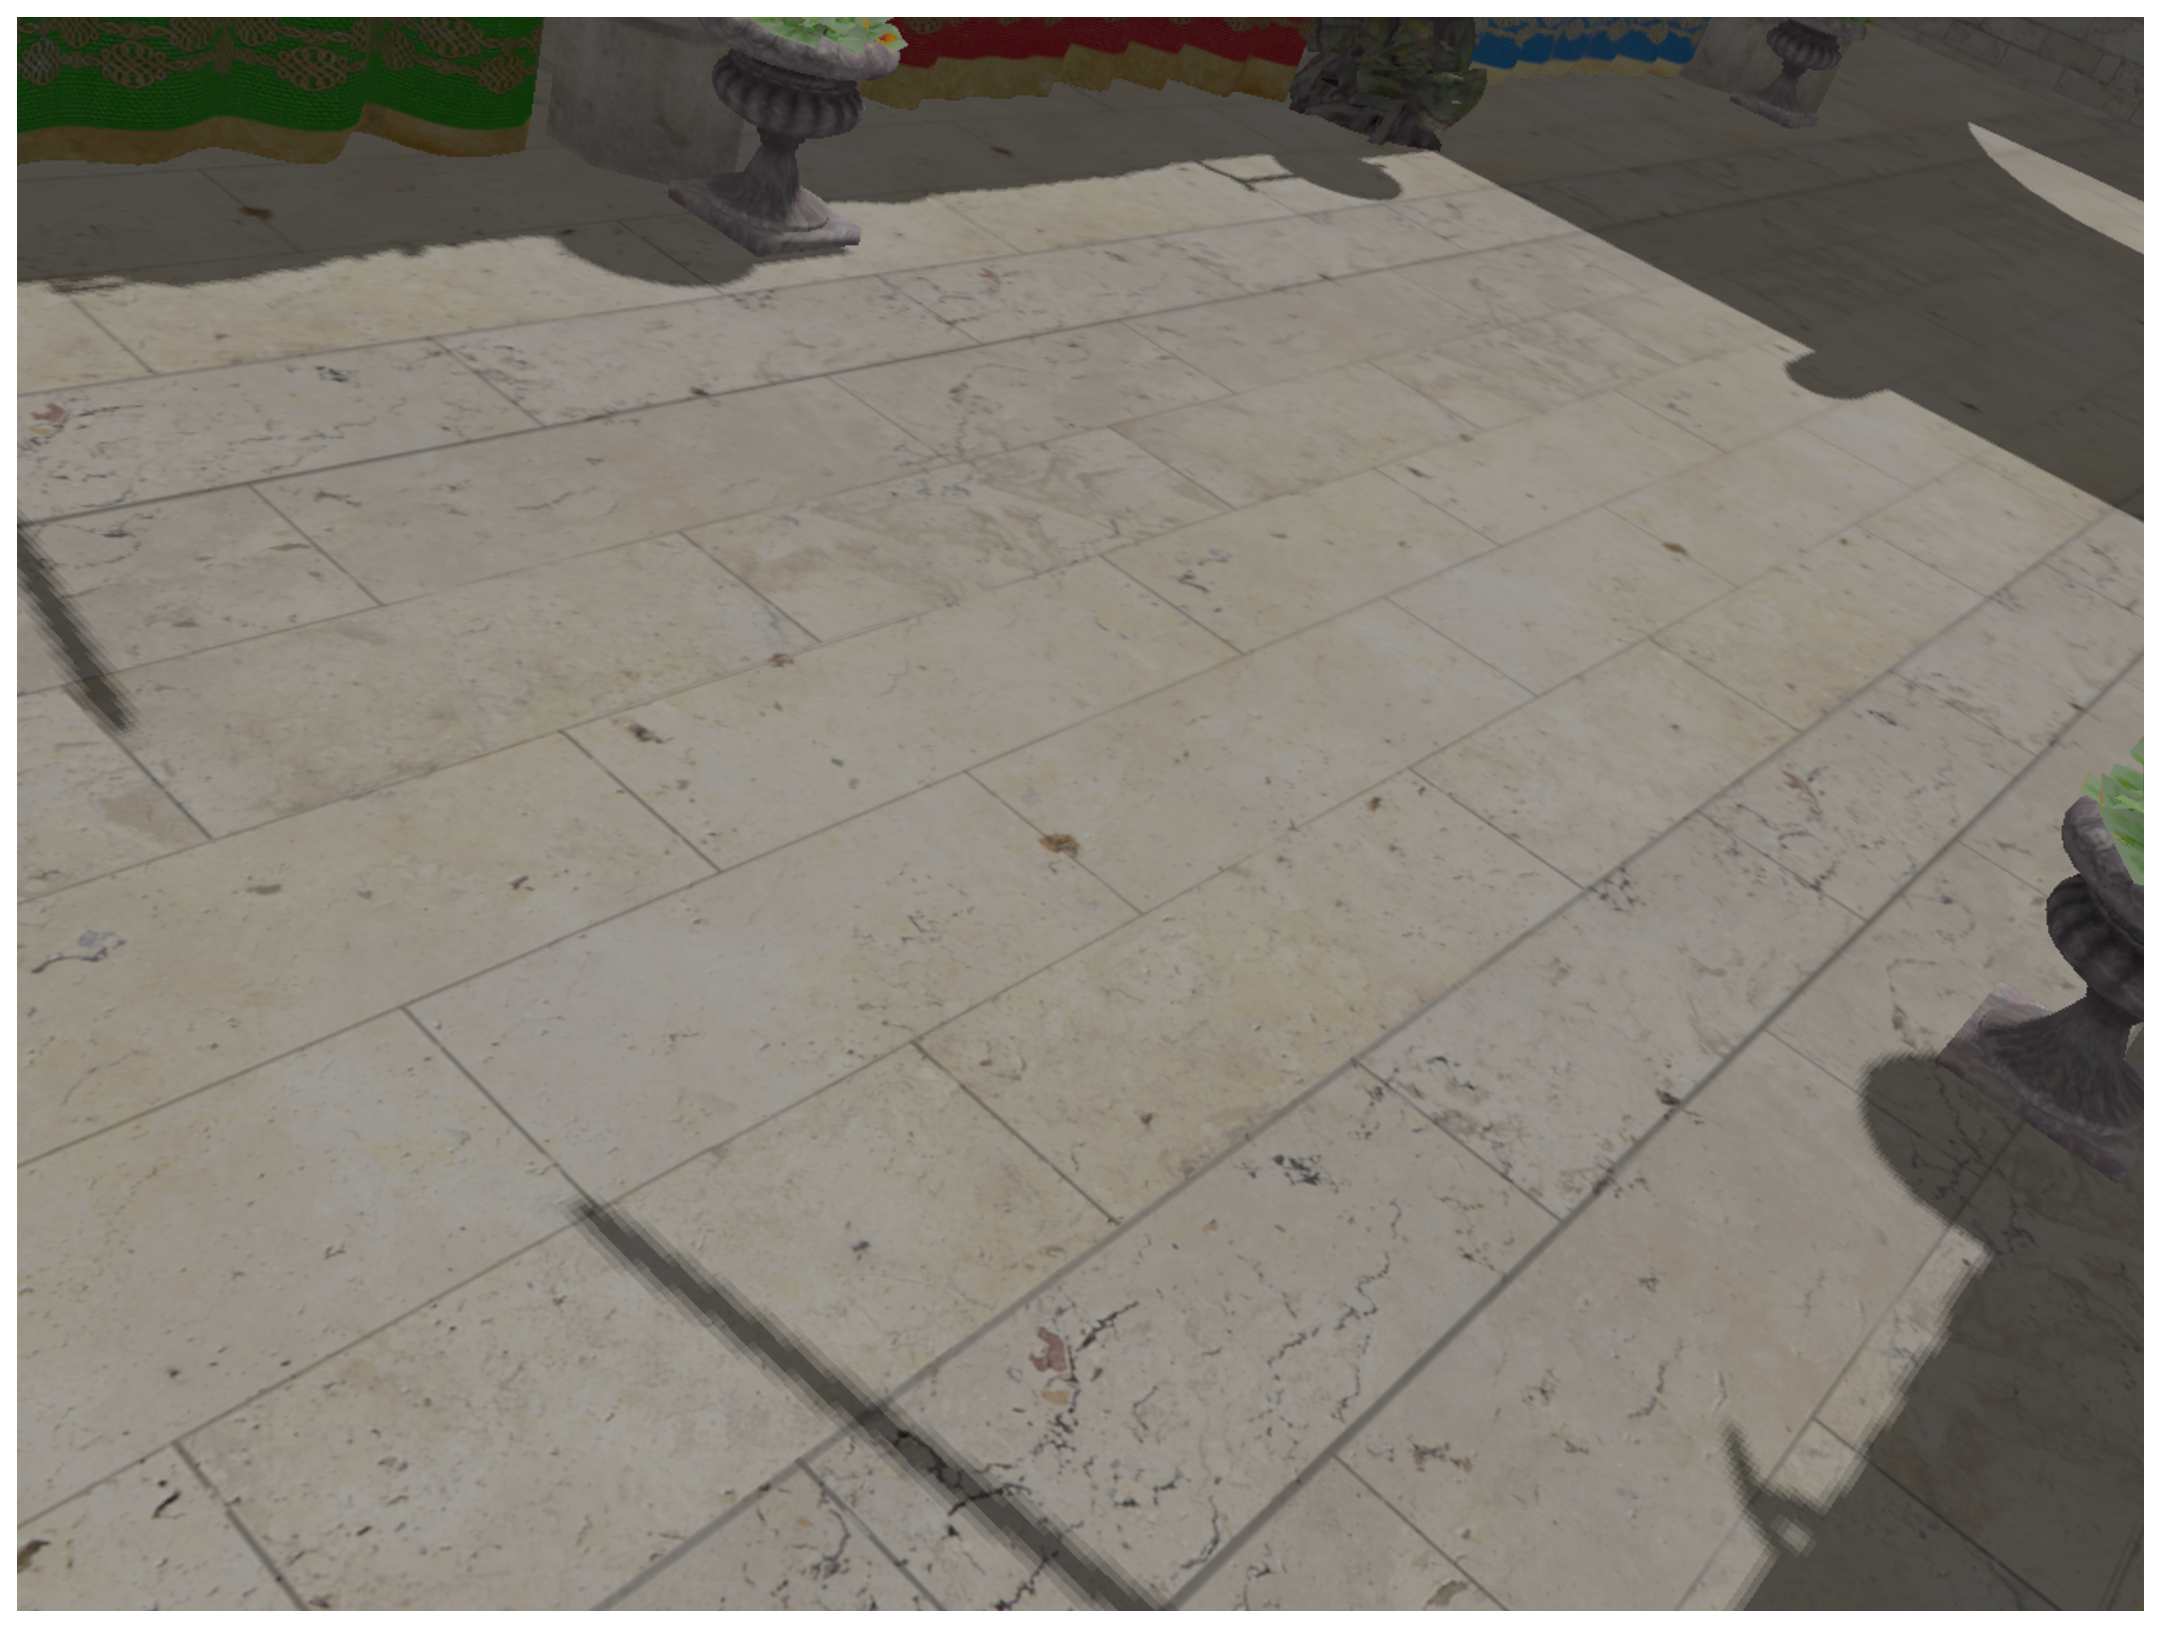
\includegraphics[width=\textwidth]{pics/shadows/shadowMapping/pcf_nearest.eps}
\end{frame}

\begin{frame}[fragile]
\frametitle{PCF}
{\small
  \begin{minted}[frame=lines]{glsl}
float shadow = 0.0;
vec2 texelSize = 1.0 / textureSize(shadowTexture, 0);
for(int x = -1; x <= 1; ++x)
{
    for(int y = -1; y <= 1; ++y)
    {
        float depth = texture(shadowTexture, 
          shadow_pos.xy + vec2(x, y) * texelSize).r; 
        shadow += shadow_pos.z - bias > depth ? 1.0 : 0.0;        
    }    
}
shadow /= 9.0;

  \end{minted}
}
\end{frame}

\begin{frame}
    \frametitle{Souhrn}
    $+$
    \begin{itemize}
        \item Rychlé
        \item Jednoduché
        \item Žádná nová geometrie
        \item Umí měkké stíny
    \end{itemize}
    \vfill
    $-$
    \begin{itemize}
        \item Všesměrová světla
        \item Omezené rozlišení textur
        \item Alias
    \end{itemize}
\end{frame}
